\newpage
{\color{gray}\hrule}
\begin{center}
\section{Caratterizzazione SiPM}
%\textbf{You can add small descriptions of what the current sections describe}
\bigskip 
{\color{gray}\hrule}
\end{center}
Per la prima parte dell'esperienza, volta allo studio di un \textit{Silicon photomultiplier} (SiPM) a 667 celle in 1.3x1.3 mm$^2$, l'apparato sperimentale impiegato è compreso nel kit CAEN di caratterizzazione dei fotomoltiplicatori al silicio e permette di fornire una risposta \textit{lineare} all'energia depositata sul rivelatore. Il kit sperimentale è composto da un'unità di alimentazione e amplificazione in tensione (PSAU) con SiPM integrato, che fornisce un segnale analogico in tensione proporzionale alla carica generata dal rivelatore; tale segnale viene acquisito da un \textit{Digitizer}, il quale lo discretizza in canali (CHN) per la successiva analisi. \\
La caratterizzazione del SiPM è stata svolta dapprima in assenza di una sorgente luminosa, cioè azzerando il numero di fotoni esterni incidenti. In questo modo è possibile isolare e analizzare il rumore intrinseco del SiPM, consistente in fluttuazioni dovute alla generazione localizzata e casuale di coppie lacuna-elettrone; tali coppie si formano per agitazione termica - ogni volta che $E_{term}>E_{gap}$ - e sono sufficienti ad innescare il singolo pixel. Successivamente si osserva il SiPM in azione in presenza di una sorgente luminosa:  tramite una fibra ottica, un \textit{LED driver} invia a bassa frequenza al SiPM  impulsi luminosi (fotoni nel violetto $\lambda= (400 \pm 14)$nm) di intensità regolabile.

\subsection{Caratterizzazione di un SiPM senza sorgente luminosa}
\subsubsection{\textit{Dark Count Rate} e \textit{Optical Cross Talk}}
Il rumore di fondo di natura termica prende il nome tecnico di \textit{dark count rate} (DCR), in quanto misurato in termini di frequenza di accensione di \textit{almeno} un pixel del SiPM in completa assenza di luce.
In condizioni di bassa intensità luminosa, quando il flusso di fotoni incidenti sul SiPM è ridotto, il DCR costituisce il principale fattore limitante la sensibilità operativa dello strumento, perciò la sua misurazione permette di impostare una soglia di rivelazione $V_{thr}$ sopra la quale\footnote{Le tensioni $V_{out}$ misurate sono negative, quindi la tensione $V_{thr}$ filtra i segnali più piccoli in valore assoluto} il segnale non è più distinguibile dal rumore. \\
Una volta impostati una tensione di alimentazione $V_{bias}$ e un \textit{gain} di amplificazione $G_{ampl}$, si visualizza lo \textit{Staircase plot} (figura \ref{fig:DCR_stair}), il quale fornisce il valore del \textit{rate} (numero di conteggi al secondo) al variare della tensione di soglia $V_{thr}$.

\begin{figure}[H]
    \centering
    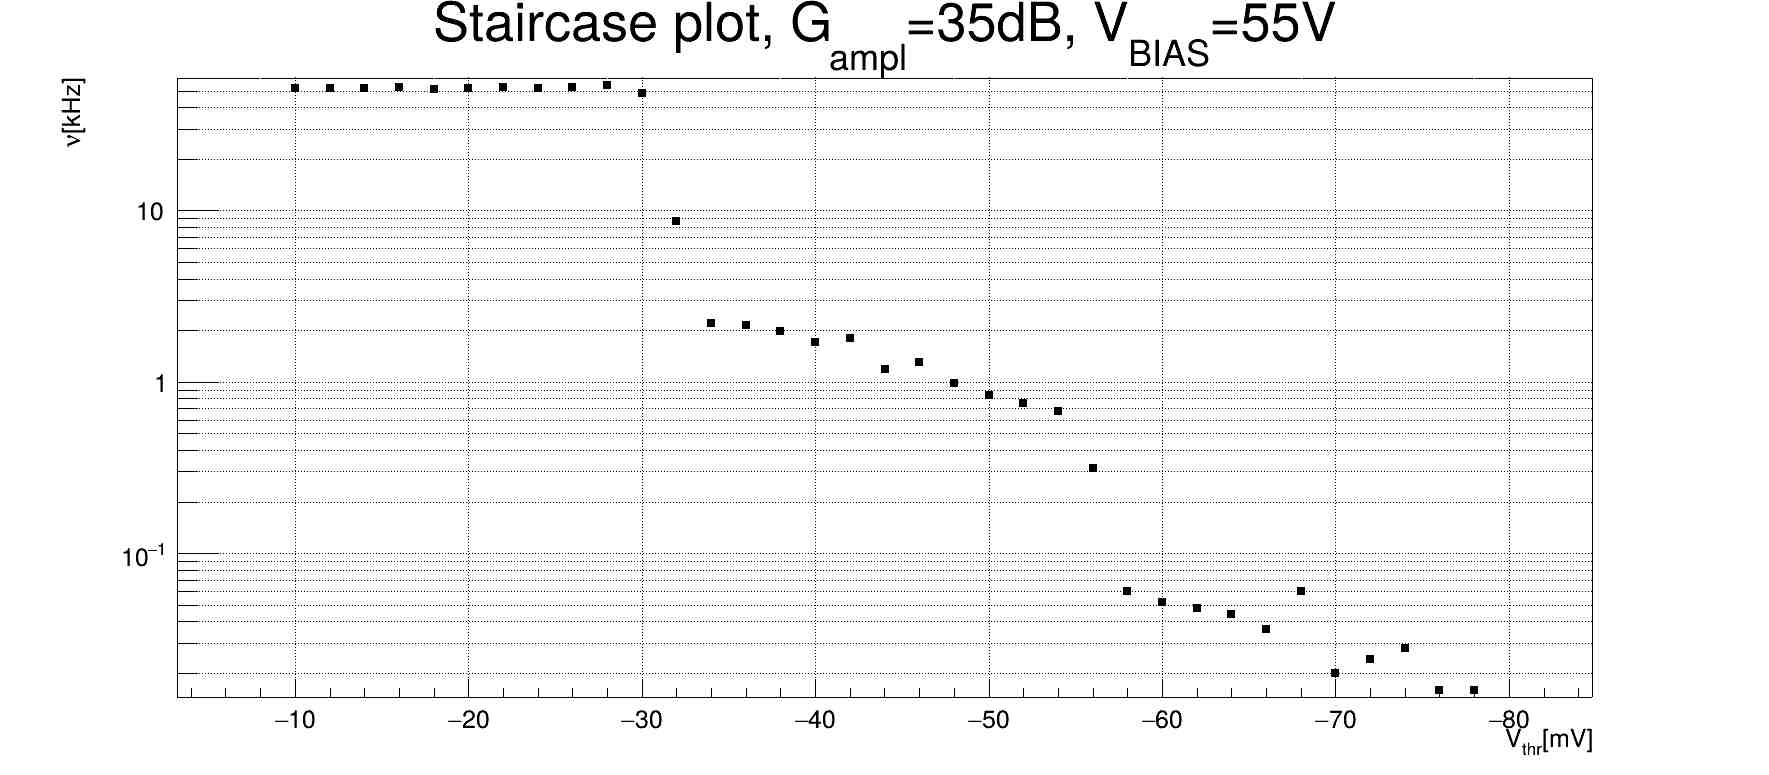
\includegraphics[width=0.82 \linewidth]{./fig1/dcr_stair.jpg}
    \caption{\footnotesize \textit{Staircase plot} a $G_{ampl}=35$dB e $V_{bias}=55$V.}
    \label{fig:DCR_stair}
\end{figure}

Dal grafico \ref{fig:DCR_stair} si osserva il caratteristico andamento a gradini: gli scalini di frequenza si collocano in corrispondenza delle tensioni $V_{out,i}$, multipli interi di $V_{out,1}$, associata a un solo pixel acceso. 

Per ottenere la miglior stima del DCR, si effettuano misure ripetute del \textit{rate} a una tensione di soglia $V_{thr} = -17$mV fissata a circa metà del primo livello e con un intervallo di tempo di acquisizione $\Delta{t}$ (\textit{gate width}) prestabilito. 
Si effettua dunque un fit gaussiano sulla distribuzione dei conteggi ottenuta, da cui vengono estratti il valore atteso $N_1$ di impulsi ricevuti nell'intervallo $\Delta{t}_1$ e la sua deviazione standard $\sigma_{N,1}$.
La miglior stima del \textit{rate}, data dal rapporto tra $N_1$ e il gate $\Delta{t}$, è 
$$\nu_1 = (51.1  \pm  0.4 ) \text{ kHz } $$
Per l'analisi dell'\textit{optical cross talk} è necessario ripetere lo stesso procedimento a fissata $V_{thr} = -44$mV (circa a metà del secondo gradino); in questo modo si ottiene la stima del \textit{rate} per il secondo livello $\nu_2$: 
$$\nu_2 = (1.23  \pm0.05 ) \text{ kHz } $$
\begin{multicols}{2}
\begin{figure}[H]
    \centering
    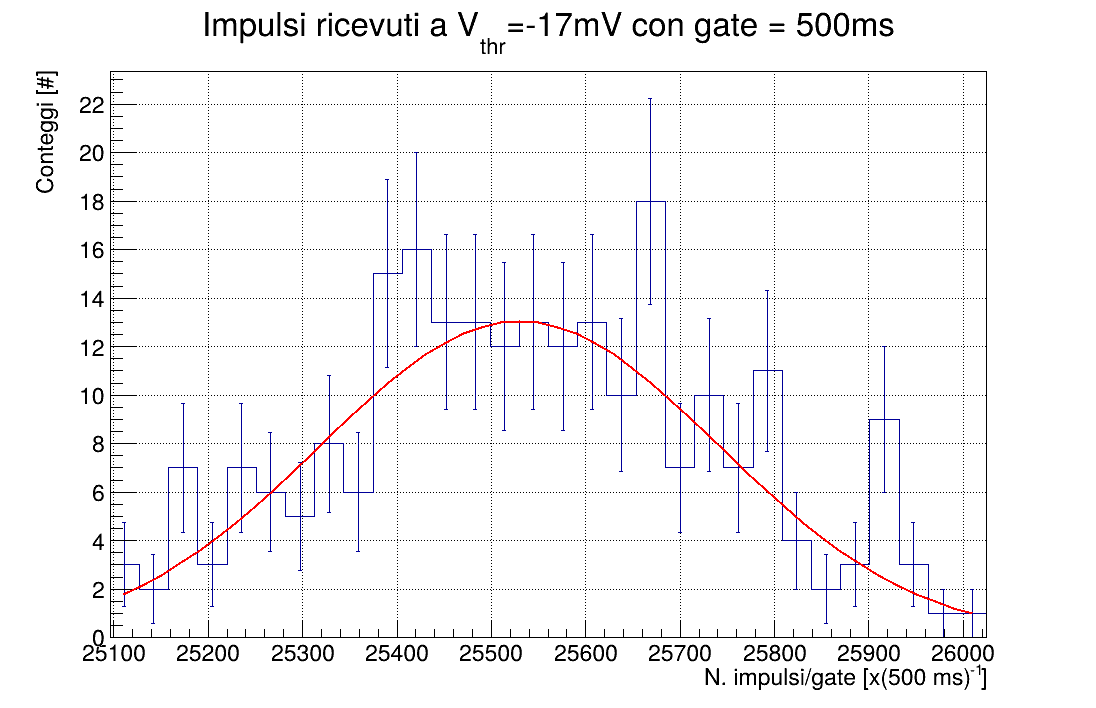
\includegraphics[width=0.99\linewidth]{./fig1/dcr_17.png}
    \caption{\footnotesize Istogramma dei conteggi per numero di impulsi ricevuti a $V_{thr}=-17$ mV e \textit{gate width} di 500 ms; in rosso è rappresentato il fit gaussiano: parametri estratti $N_1= (25530 \pm  16) $CHN e $\sigma_{N,1}= ( 211 \pm  15 ) \text{CHN}$, $\chi^2=23.7$ e 27 d.o.f.}
\end{figure}

\begin{figure}[H]
    \centering
    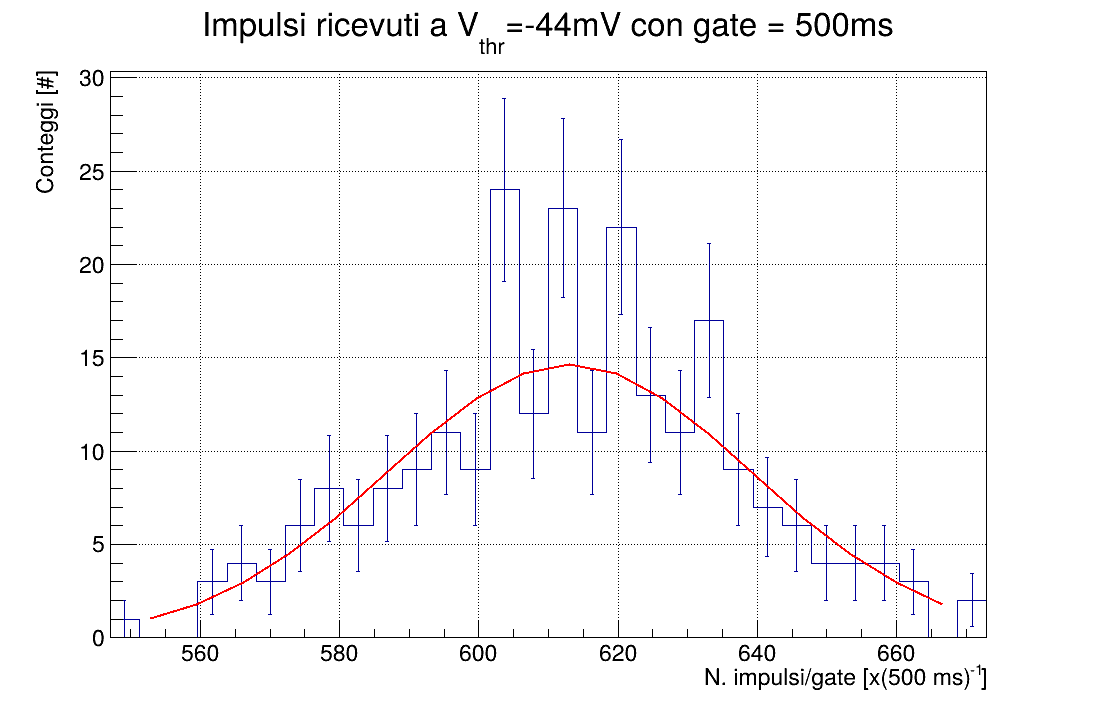
\includegraphics[width=0.99\linewidth]{./fig1/dcr_44.png}
    \caption{\footnotesize Istogramma dei conteggi per numero di impulsi ricevuti a $V_{thr}=-44$ mV e \textit{gate width} di 500 ms; in rosso è rappresentato il fit gaussiano: parametri estratti $N_2= ( 613 \pm  2) \text{ CHN }$ e $\sigma_{N,2}= ( 26 \pm  2 ) \text{ CHN }$, $\chi^2=19.0$ e 23 d.o.f.}
\end{figure}
\end{multicols}

\textit{Osservazione.} È stato possibile stimare soltanto i \textit{rate} dei primi due livelli $\nu_1$ e $\nu_2$ poichè, come evidenziato dal grafico \ref{fig:DCR_stair}, lo strumento non è sensibile alle frequenze troppo basse.




L'\textit{optical cross talk} (OCT) è definito come il rapporto tra il \textit{rate} corrispondente all’accensione di \textit{almeno due} celle $\nu_2$ e il rate misurato all’accensione di \textit{almeno una} singola cella $\nu_1$, $$OCT = \frac{\nu_2}{\nu_1}$$
ed è conseguenza del fatto che la valanga di carica prodotta da una cella può scatenarne un'altra in una cella vicina.
\\
Utilizzando le stime di $\nu_1$ e $\nu_2$ si ricava la frazione di eventi in cui è avvenuto l'\textit{optical cross talk}.
$$ OCT = (2.4  \pm0.1  ) \text{ \% } $$
Questa stima è in linea con il valore atteso per SiPM con queste caratteristiche.
\subsubsection{DCR e OCT in funzione della temperatura del sistema}
In questa sezione si analizza il comportamento del DCR e dell'OCT al variare della temperatura \textit{T} del sistema, prima del raggiungimento della condizione di stabilità termica del SiPM.\\
Subito dopo aver acceso il SiPM, sono stati raccolti sette volte i valori della temperatura e le due distribuzioni di conteggi per numero di impulsi ricevuto, una a fissata $V_{thr,1}$ per il primo gradino e l'altra a fissata $V_{thr,2}$ per il secondo gradino\footnote{La tesione di soglia $V_{thr}$ è stata sempre scelta circa a metà del gradino}. In appendice 5.1 vengono riportati gli istogrammi delle due distribuzioni e i relativi fit gaussiani per il calcolo di DCR e OCT.
\begin{table}[H]
    \centering
    \begin{tabular}{|c|c|c|c|}
        \hline
        
        \textbf{T[$^o$C]} & \textbf{$\mathbf{\nu_1}$ (DCR)[kHz]} & \textbf{$\mathbf{\nu_2}$ [kHz]} & \textbf{OCT=$\mathbf{\nu_2/\nu_1}$ [\%]} \\ \hline
        
        $20.4  \pm  0.5 $  &  $16.6  \pm  0.2  $  &  $ 0.27 \pm  0.02 $  &  $1.63  \pm  0.13 $ \\ \hline
        $22.1  \pm  0.3 $  &  $17.59  \pm  0.18  $  &  $0.29  \pm  0.5 $  &  $1.7  \pm  0.3 $ \\ \hline
        $22.7  \pm  0.2 $  &  $18.4  \pm  0.3  $  &  $0.276  \pm  0.012 $  &  $1.50  \pm  0.07 $ \\ \hline
        $23.0  \pm  0.1 $  &  $19.1  \pm  0.2  $  &  $0.29  \pm  0.02 $  &  $1.52  \pm  0.11 $ \\ \hline
        $23.4 \pm  0.1 $  &  $19.7  \pm  0.2  $  &  $0.29  \pm  0.02 $  &  $1.49  \pm  0.11 $ \\ \hline
        $23.7  \pm  0.1 $  &  $20.20  \pm  0.19  $  &  $0.30  \pm  0.03 $  &  $1.50  \pm  0.13 $ \\ \hline
        $23.9  \pm  0.1 $  &  $20.75  \pm  0.16  $  &  $0.293  \pm  0.019 $  &  $1.41  \pm  0.09 $ \\ \hline
        
    \end{tabular}
    \caption{\footnotesize Valori di temperatura del sistema $T$, \textit{rate} $\nu_1$ (DCR), \textit{rate} $\nu_2$ e OCT=$\nu_2$/$\nu_1$ alla tensione $V_{bias}=55$V e \textit{gain} $G_{ampl}=35$dB.}
    \label{tab:temp}    
\end{table}

\textit{Osservazione.} Siccome non è possibile acquisire i due istogrammi simultaneamente e la temperatura del SiPM varia velocemente, molte coppie di istogrammi sono in realtà riferite a due valori diversi di temperatura, $T_1$ e $T_2$, di cui si è calcolata la media e la semidispersione.

Separatamente vengono graficate le coppie di valori ($T_j$,$DCR_j$) e ($T_i$,$OCT_i$) e si effettua su ciascun grafico una regressione lineare sui dati, dimostrando che il DCR dipende linearmente dalla temperatura, mentre l'OCT è costante rispetto a questa.
Infatti, dall'analisi sperimentale risulta che il coefficiente angolare $a$ della retta $DCR$ in funzione di $T$, il cui valore è $a= ( 1.8 \pm  0.2 ) \text{kHz/}^o\text{C}$, risulta positivo e significativamente diverso da zero; mentre il coefficiente angolare $c$ della retta $OCT$ in funzione di $T$, il cui valore è $c= (-0.08  \pm  0.09 ) ^o\text{C}^{-1}$, risulta statisticamente compatibile con zero.
\begin{multicols}{2}
\begin{figure}[H]
    \centering
    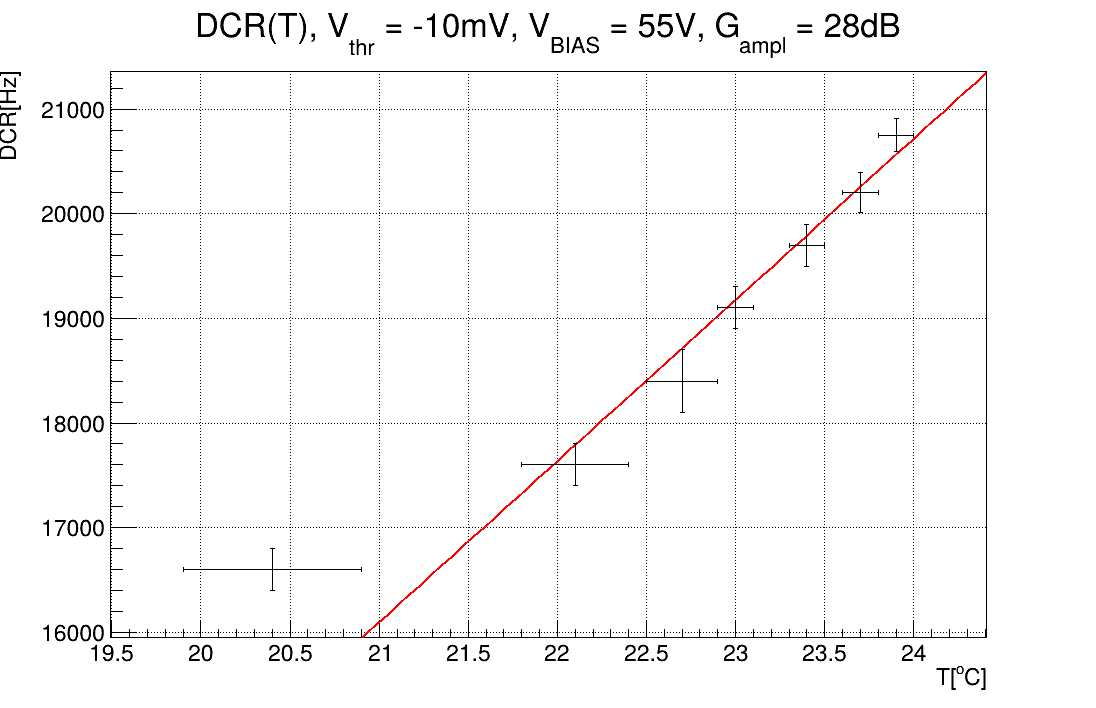
\includegraphics[width=0.99\linewidth]{fig1/DCRT.png}
    \caption{\footnotesize Grafico delle coppie ($T_j$,$DCR_j$) e fit lineare $y = ax+b$: parametri estratti $a= (1.54 \pm  0.19 ) \text{kHz/}^o\text{C}$ e $b= (-16  \pm  5 ) \text{kHz}$, $\chi^2=4.9$, d.o.f.$=5$.}
    \label{fig:DCR_T}
\end{figure}

\begin{figure}[H]
    \centering
    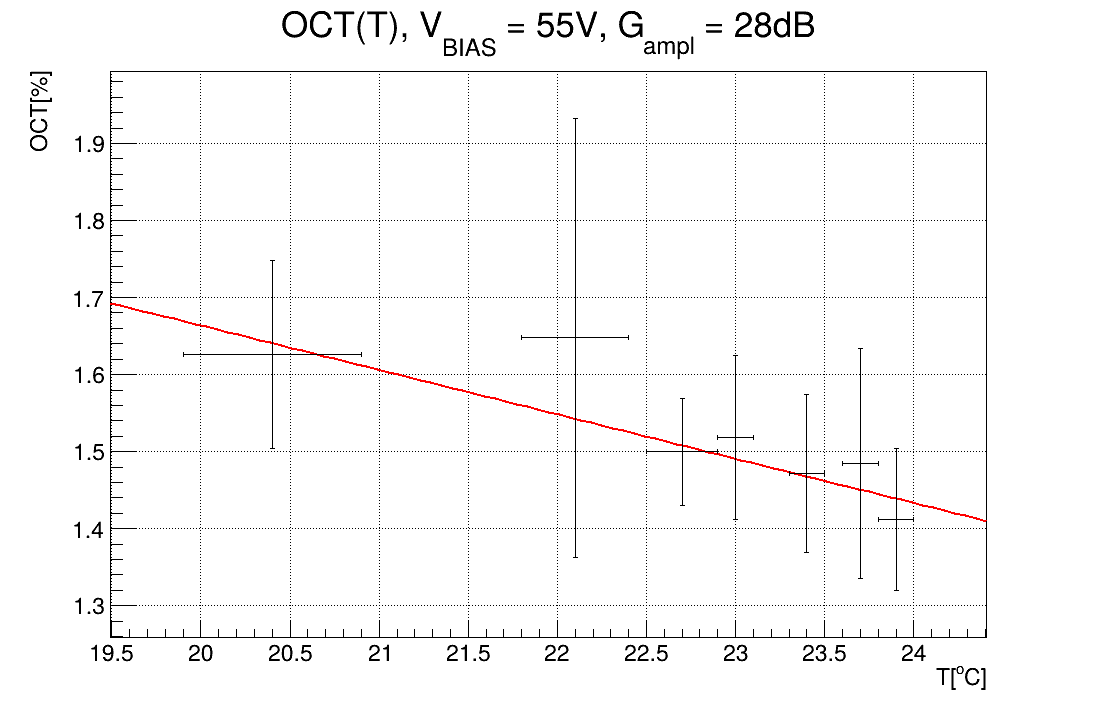
\includegraphics[width=0.99\linewidth]{fig1/OCTT.png}
    \caption{\footnotesize Grafico delle coppie ($T_i$,$OCT_i$) e fit lineare $y=cx+d$: parametri estratti $c= (-0.06  \pm  0.04 ) ^o\text{C}^{-1}$ e $d= (2.8  \pm  1.0 ) \text{\%}$, $\chi^2=0.4$, d.o.f.$=5$.}
    \label{fig:OCT_T}
\end{figure}
\end{multicols}
Per il fit dell'OCT, il valore di $\chi^2$ è molto minore del numero di gradi di libertà e questo risultato è dovuto a due fattori: in primo luogo, visto che la variazione di $T$ è avvenuta molto velocemente, le incertezze sui valori della temperatura sono abbastanza grandi; d'altra parte, anche le incertezze sui \textit{rates} risultano elevate, in quanto, per la necessità di prendere velocemente le misure, si è dovuto impostare un \textit{gate} di acquisizione abbastanza corto (500ms).

\textit{Osservazione.} Il risultato suggerisce dunque che al crescere della temperatura del sistema aumenta la probabilità che per agitazione termica si inneschi una valanga, mentre non aumenta significativamente la probabilità che la valanga di una cella accenda altre celle adiacenti.

\subsection{Caratterizzazione di un SiPM con sorgente luminosa (LED)}

Si introduce ora una sorgente luminosa (LED con $\lambda= (400 \pm 14)$nm) e si sfrutta un trigger esterno che dà inizio alla lettura ogni volta che il LED invia un impulso di luce; in questo modo non verranno conteggiati eventi dovuti al rumore intrinseco ma verranno anche conteggiate le letture nulle.

\textit{Osservazione.} Con un trigger interno, il DCR ($\nu_1 \sim 50$ kHz) avrebbe influenzato significativamente la misura, richiedendo la sottrazione dai conteggi corrispondenti all'accensione di una cella di un valore pari a $\nu_1\tau$, con $\tau\sim120$s tempo totale di acquisizione. Il trigger esterno invece permette di annullare il DCR, ma non l'OCT, il quale però è solo dell'ordine del $2\%$.

\subsubsection{Prima stima di $G_\text{SiPM}$}
Dal momento che la carica restituita da una cella attivata da un fotoelettrone viene amplificata dalla PSAU di un fattore $G_{ampl}$ espresso in unità naturali\footnote{Relazione di conversione: $G_{ampl}(dB)=20\log_{10}G_{ampl}$}, la carica totale prodotta da un singolo impulso luminoso $q_{1-cella}$ è pari a $$q_{1-cella}=G_\text{ampl}G_\text{SiPM}e$$ 
Fissati una tensione di alimentazione $V_{bias}$, un \textit{gain} di amplificazione $G_{ampl}$ e l'intensità del LED, si visualizza sul Digitizer il caratteristico spettro dei fotoelettroni riportato in figura \ref{fig:LED_Gsipm}.

\begin{figure} [H] 
    \centering
    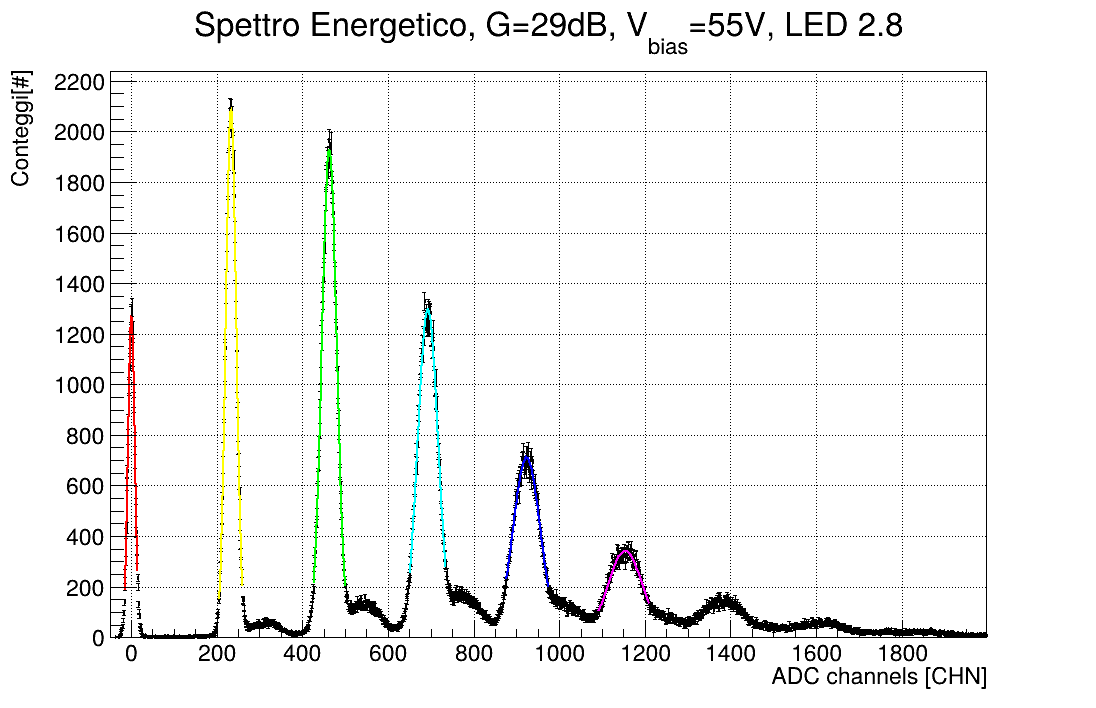
\includegraphics[width=0.60\linewidth]{fig1/led_gsipm.png}
    \caption{ \footnotesize Istogramma dei conteggi per numero di canale a $V_{BIAS}=55$V, $G_{ampl}=29$dB, intensità del LED di 2.8. e fit gaussiani ditinguibili dal colore (per ciascun fit parametri estratti, d.o.f e $\chi^2$ sono riportati nella tabella \ref{tab:gsipm} in appendice)}
    \label{fig:LED_Gsipm}
\end{figure}

\textit{Osseravzione.} Ciascun picco del grafico \ref{fig:LED_Gsipm} rappresenta un diverso numero di celle accese e la sua altezza rappresenta la quantità di volte in cui ciò avviene: in particolare, il primo rappresenta gli eventi in cui il trigger si è attivato, ma non si sono rilevati fotoni, mentre i successivi rappresentano 1, 2,... fotoni incidenti.

Inoltre, è possibile notare che i picchi sono equidistanti di $\Delta_{pp}$, corrispondente alla carica raccolta da una singola cella. Effettuando dei fit guassiani sui primi 6 picchi, da cui si estraggono i valori attesi $p_i$ e le rispettive deviazioni standard $\sigma_{p,i}$ (vedi Tabella \ref{tab:gsipm} in appendice), si possono calcolare diverse stime $\Delta_{pp, i}$ tra picchi consecutivi. Dopo aver dimostrato che queste appartengono alla stessa popolazione tramite test di Gauss, se ne fa una media pesata ottenendo $$ \langle\Delta_{pp}\rangle= (231  \pm  11 ) \text{CHN} $$
Noto il fattore di calibrazione del sistema, $k=40$ fC/CHN, la carica totale restituita da una cella $q_{1-cella}$ si può esprimere anche come $$q_{1-cella}=k\langle\Delta_{pp}\rangle$$
In conclusione, si può ottenere una prima stima del guadagno del SiPM dalla seguente formula 
\begin{equation}
    G_{SiPM}=\frac{k\Delta_{pp}}{G_{ampl}e}= (2.05  \pm  0.09 )\cdot10^6
    \label{eq:GSiPM}
\end{equation}
\textit{Osservazione.} Come ci si aspetta per il modo di funzionamento a valanga, $G_{SiPM}$ è dell'ordine di $10^6$. 

\subsubsection{Verifica della linearità dell'amplificazione della carica}
In questa sezione, si vuole dimostrare che l'intensità del segnale associata all'accensione di una singola cella $\Delta_{pp}$ cresce linearmente con l'amplificazione $G_{ampl}$; perciò a intensità del LED di 2.5 e $V_{bias}=55$V fissate, si acquisiscono gli spettri dei fotoelettroni al variare di $G_{ampl}$. \\
Da ogni spettro si ricavano le rispettive stime di $\langle\Delta_{pp}\rangle_j$ e le relative incertezze (riportate in tabella \ref{tab:gain}) seguendo lo stesso procedimento descritto nel paragrafo precedente 1.2.1. Tutti gli spettri sono riportati nell'appendice \ref{sec:app_gain}.

\begin{multicols}{2}
\begin{figure} [H]
    \centering
    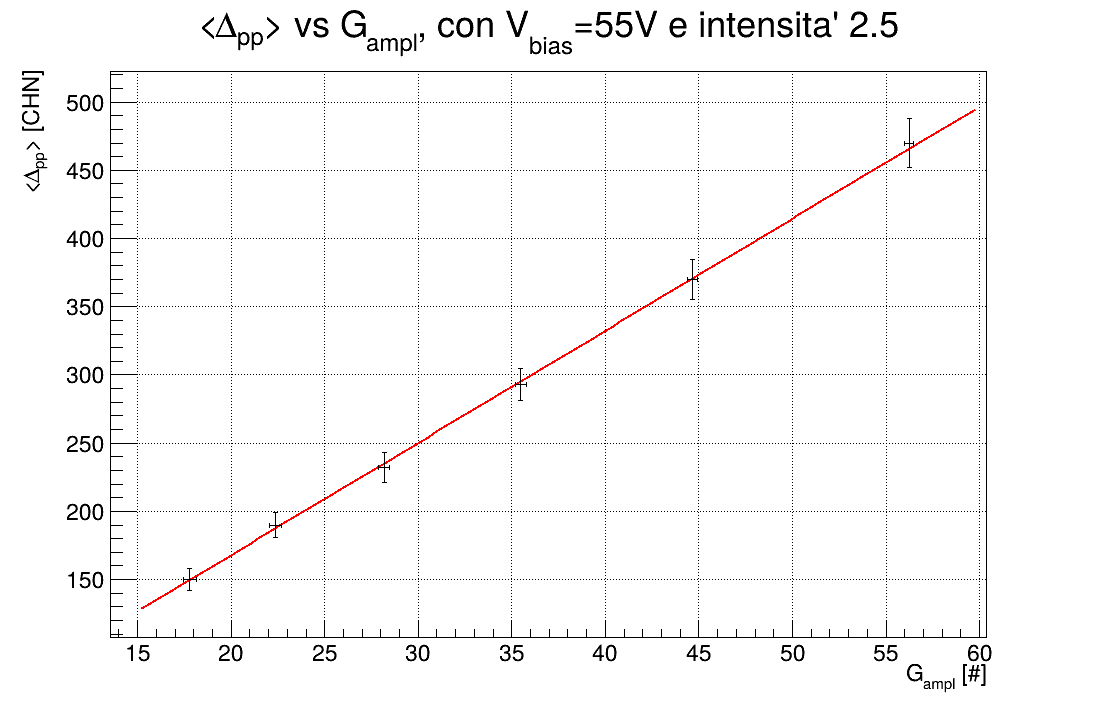
\includegraphics[width=1. \linewidth]{fig1/deltapp_G.png}
    \caption{ \footnotesize Coppie di dati ($G_{ampl,j}$,$\langle\Delta_{pp}\rangle_j$) e regressione lineare con $\chi^2=0.2$ e d.o.f.$=4$.}
    \label{fig:deltapp_G}
\end{figure}

\begin{table}[H]
    \bigskip
    \centering
     \begin{tabular}{|c|c|}
        \hline
        \textbf{$\mathbf{\langle\Delta_{pp}\rangle}$[CHN]} & \textbf{$\mathbf{G_{ampl}}$[dB]} \\ \hline
        $150 \pm 8$                                    & $25 \pm 1$                         \\ \hline
        $190 \pm 9$                                    & $27 \pm 1$                         \\ \hline
        $232 \pm 11$                                    & $29 \pm 1$                         \\ \hline
        $293 \pm 12$                                    & $31 \pm 1$                         \\ \hline
        $370 \pm 15$                                    & $33 \pm 1$                         \\ \hline
        $470 \pm 18$                                    & $35 \pm 1$                         \\ \hline
    \end{tabular}
    \caption{\footnotesize Valori di \textit{gain} di amplificazione e distanza picco-picco media $\langle\Delta_{pp}\rangle_j$ alla tensione $V_{bias}=55$V e con intensità LED 2.5.}
    \label{tab:gain}
\end{table}

\end{multicols}
Dal grafico \ref{fig:deltapp_G} delle coppie di dati ($G_{ampl,j}$,$\langle\Delta_{pp}\rangle_j$) si evince una dipendenza lineare di $\langle\Delta_{pp}\rangle_j$ con il \textit{gain} di amplificazione del tipo $\langle\Delta_{pp}\rangle_j=a \cdot G_{ampl,j}+b$. I valori estratti dal fit lineare risultano: $ a =  (8.2  \pm  0.4 ) \text{CHN} $ e $ b = (4  \pm  13)$CHN.

Il valore di $\chi^2 = 0.2$ del fit è molto piccolo rispetto al numero di gradi di libertà; questo è da attribuirsi al fatto che per stimare le posizioni dei picchi dei vari spettri energetici si sono utilizzate le deviazioni standard delle singole gaussiane $\sigma_{p,i}$ come errori sulle medie delle stesse: gli errori relativi, specialmente nei picchi a valori di CHN maggiori, risultano quindi piuttosto grandi.

Il parametro $a$ ottenuto dal fit lineare risulta compatibile tramite test di Gauss con quello che si ricava da $ a = \frac{G_\text{SiPM}\cdot e}{k} = (8.21  \pm  0.04 ) \text{ CHN }$ dalla relazione \ref{eq:GSiPM}, usando il valore di $G_{SiPM}$ stimato nella sezione precedente (equazione \ref{eq:GSiPM}). La compatibilità statistica assicura dunque che il coefficiente angolare della retta di fit ha il significato fisico atteso. \\
Allo stesso modo, il valore di $b$ ottenuto risulta statisticamente compatibile con zero.

\textit{Osservazione.} I risultati appena ottenuti, a meno di una costante moltiplicativa, hanno permesso di dimostrare che la carica totale restituita all'accensione di una singola cella,\\$q_{1-cella}=k\langle\Delta_{pp}\rangle$, aumenta linearmente con il \textit{gain} di amplificazione regolabile dalla \textit{PSAU}.

\subsubsection{$G_\text{SiPM}$ in funzione della tensione $V_\text{bias}$}
Al fine di poter studiare l'andamento del guadagno del SiPM $G_{SiPM}$ in funzione di $V_{bias}$ vengono mantenuti costanti l'intensità del LED a 2.5 e il \textit{gain} di amplificazione a $29$dB.\\
Sperimentalmente è possibile ripetere la stessa procedura vista nel paragrafo precedente per l'ottenimento delle stime di $\langle\Delta_{pp}\rangle$ da ogni spettro e dunque stimare il $G_{SiPM}$ usando la relazione \ref{eq:GSiPM} al variare della tensione $V_{bias}$. In appendice 5.2.3 sono riportati tutti gli spettri di fotoelettroni. \\
Si ottengono così cinque coppie di valori di ($G_{SiPM,k}$, $V_{bias,k}$), riportate in tabella \ref{tab:vbias}, le quali suggeriscono un andamento lineare e crescente; per verificare tale ipotesi, si è effettuata una regressione lineare sui dati, riportata in figura \ref{fig:vbias_G}.

\begin{multicols}{2}
\begin{figure} [H]
    \centering
    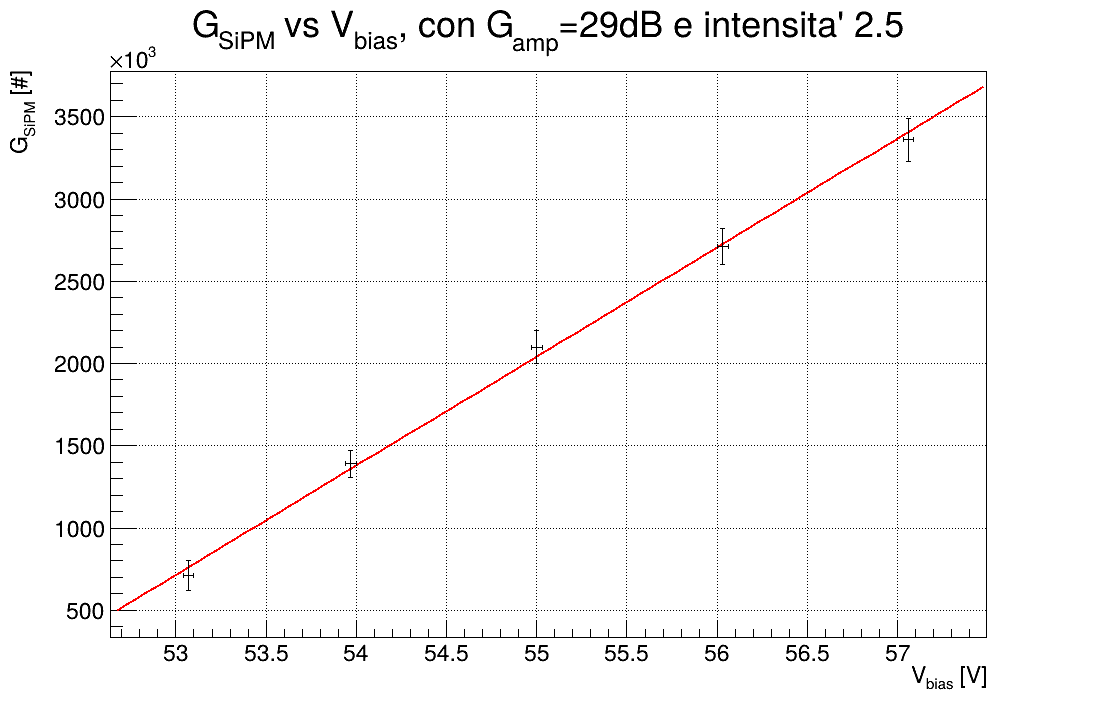
\includegraphics[width=.94\linewidth]{fig1/led_vbias.png}
    \caption{ \footnotesize Coppie di valori ($V_{bias,j}$, $G_{SiPM,j}$) e regressione $G_{SiPM}=a+b\cdot V_{bias}$ con parametri restituiti $a= ( 6.6 \pm 0.3 )\cdot10^5 \text{ V }^{-1}$, $b = (-3.45\pm0.18)\cdot10^7$, $\chi^2=0.7$ e d.o.f.$=3$}
    \label{fig:vbias_G}
\end{figure} \phantom{.}

\begin{table}[H]
\centering
    \begin{tabular}{|c|c|}
    \hline
    $\mathbf{G_\textbf{SiPM}}$\textbf{[\#]} & $\mathbf{V_\textbf{bias}}$\textbf{[V]} \\
    \hline
    $ (710 \pm 90)\cdot 10^3 $ &$ 53.07 \pm 0.03$ \\
    \hline
    $ (1.39 \pm 0.08)\cdot 10^6$ &$ 53.97 \pm 0.03$ \\
    \hline
    $ (2.1 \pm 0.1)\cdot 10^6$ &$ 55.00 \pm 0.03$ \\
    \hline
    $ (2.71 \pm 0.11)\cdot 10^6$ &$ 56.03 \pm 0.03$ \\
    \hline
    $ (3.36 \pm 0.13)\cdot 10^6$ &$ 57.06 \pm 0.03$ \\
    \hline
    \end{tabular}
    \caption{ \footnotesize Valori di guadagno del SiPM $G_{SiPM}$ e tensione di alimentazione $V_{bias}$ a intensità del LED di 2.5 e $G_{ampl}=29$dB fissati}
    \label{tab:vbias}
\end{table}
\end{multicols}
Come nel fit lineare precedente, il valore di $\chi^2 = 0.7$ risulta molto basso e una possibile causa è la grande incertezza sulle medie dei picchi degli spettri energetici.

\textit{Osservazione.} L'andamento crescente con la tensione di alimentazione è spiegabile con il fatto che aumentando la tensione di polarizzazione inversa delle celle aumenta la portata della valanga e dunque il guadagno del SiPM. \\

\subsubsection{Stima del numero di fotoni $\mu_{ph}$ rivelati in funzione dell'intensità del LED}

Si determina infine il numero medio di celle del SiPM colpite per 3 diverse intensità luminose del LED, mantenendo costanti la tensione di alimentazione $V_{bias} = 55$V e l'amplificazione della PSAU $G_{ampl} = 29$dB. 

\begin{figure} [H]
    \centering
    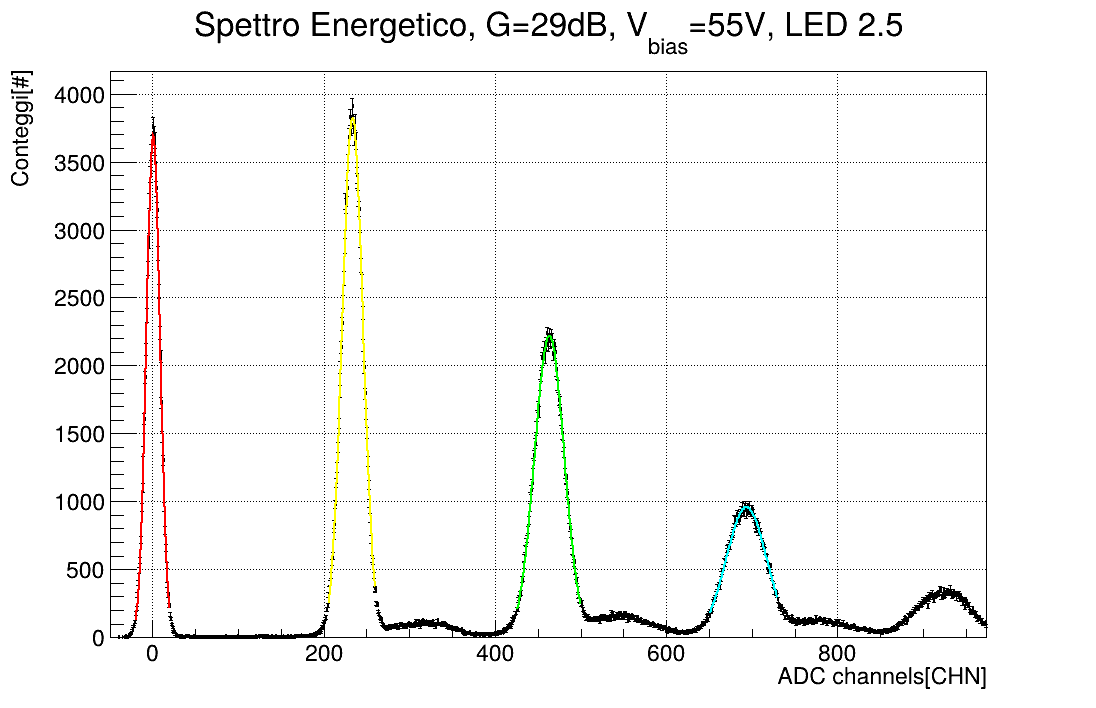
\includegraphics[width=.65\linewidth]{fig1/led_2_5.png}
    \caption{ \footnotesize Istogramma dei conteggi per numero di canale a $V_{BIAS}=55$V, $G_{ampl}=29$dB, intensità del LED di 2.5. e fit gaussiani distinguibili dal colore (per ciascun fit d.o.f e $\chi^2$ sono riportati nella tabella \ref{tab:led2_5} in appendice)}
    \label{fig:led_I_2_5}
\end{figure}

Il numero medio di fotoelettroni può essere stimato in due modi, uno più approssimativo e uno più accurato.

Il metodo approssimativo consiste nello stimare la media dell'istogramma $\langle CHN\rangle$ e la distanza media tra i picchi $\langle\Delta_{pp}\rangle$: il numero medio di fotoelettroni è stimato dal rapporto
$$\mu_{ph} = \frac{\langle CHN\rangle}{\langle\Delta_{pp}\rangle}$$
Nella tabella \ref{tab:I} di seguito sono riportate le stime di $\langle CHN\rangle$, $\langle\Delta_{pp}\rangle$ e $\mu_{ph}$ al variare dell'intensità del LED.

\begin{table}[H]
\centering
    \begin{tabular}{|c|c|c|c|}
    \hline
    $\mathbf{I_{LED}}$ & $\mathbf{\langle \Delta_{pp}\rangle}$ \textbf{[CHN]} & $\mathbf{\langle CHN \rangle} $\textbf{[CHN]} &$ \mathbf{\mu_{ph}}$ \\
	\hline
    $2.0$ &$ 232.60\pm0.04 $ &$191.1\pm0.3$ &$0.8216\pm0.0014$ \\
    \hline
    $2.5$ &$231.71\pm0.04$ &$379.4\pm0.4$ &$1.6375\pm0.0018$ \\
    \hline
    $2.8$ &$231.02\pm0.05$ &$675.0\pm0.6$ &$2.922\pm0.003$ \\
    \hline
    \end{tabular}
    \caption{\footnotesize Valori di $\langle CHN\rangle$, $\langle\Delta_{pp}\rangle$ e $\mu_{ph}$ al variare di $I_{LED}$; gli spettri per $I_{LED} = 2.0$ e $I_{LED} = 2.8$ si possono trovare in appendice 5.2.4}
    \label{tab:I}
\end{table}
Il metodo accurato consiste invece nel calcolare l'area $A_N$ sottesa a ciascun fit gaussiano, che corrisponde al numero di volte in cui si sono accese $N$ celle contemporaneamente, e associarla tramite un istogramma al numero di picco $N$; dato il basso numero punti a disposizione, l'andamento di questo istogramma è poissoniano e da un fit su di esso si estrae la stima di $\mu_{ph}$.

Per i tre spettri acquisiti al variare di $I_{LED}$, queste regressioni non vanno a buon fine a causa del limitato numero di gradi di libertà (causato dal ridotto numero di picchi) e della sottostima delle incertezze sulle aree degli integrali, in quanto esse derivano dalle incertezze sui parametri dei fit.

Per ciascun valore di $I_{LED}$ si verifica inoltre la relazione, prevista dalla teoria, tra le varianze dei picchi gaussiani
$$ \sigma^2_{N} = \sigma^2_{0} + N\sigma^2_{p} $$
in cui $\sigma_0^2$ è la varianza del picco corrispondente a 0 fotoelettroni, N è il numero di picco e $\sigma^2_p$ è una costante.
\begin{multicols}{2}
    \begin{figure} [H]
    \centering
    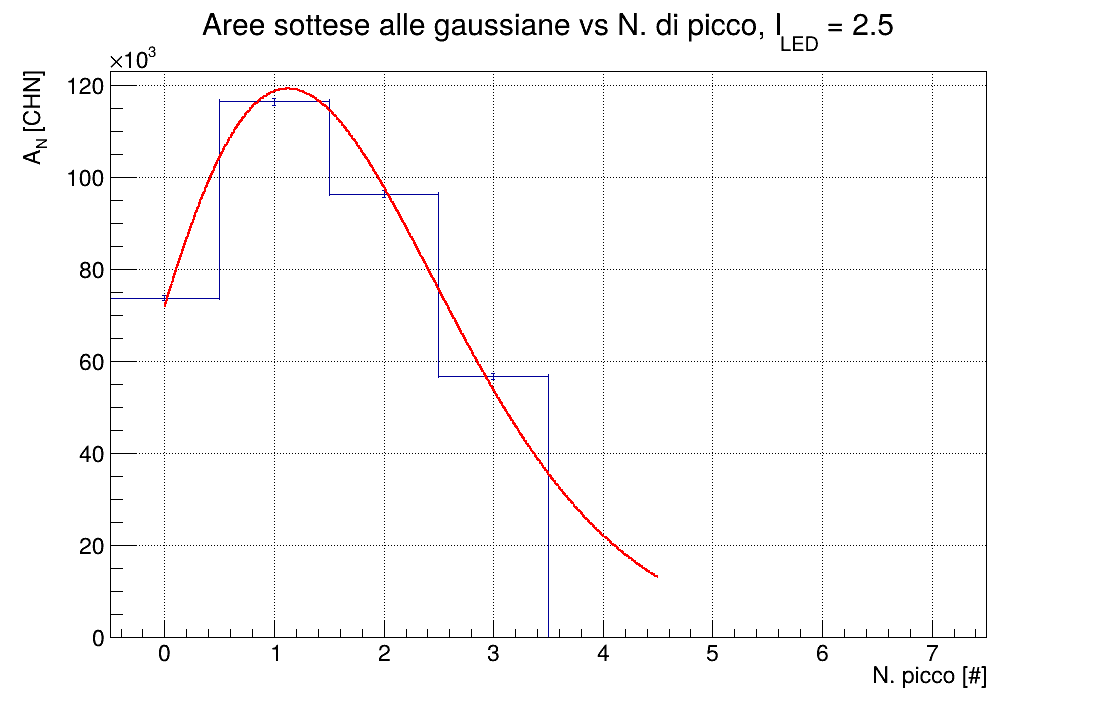
\includegraphics[width=1.\linewidth]{fig1/led_area_2_5.png}
    \caption{ \footnotesize Istogramma delle aree sottese alle gaussiane per lo spettro a $I_{LED} = 2.5$ in funzione del numero di picco con fit Poissoniano non convergente, $\chi^2 = 42$ e d.o.f$=2$.}
    \label{fig:led_pois_2_5}
\end{figure}
\begin{figure} [H]
    \centering
    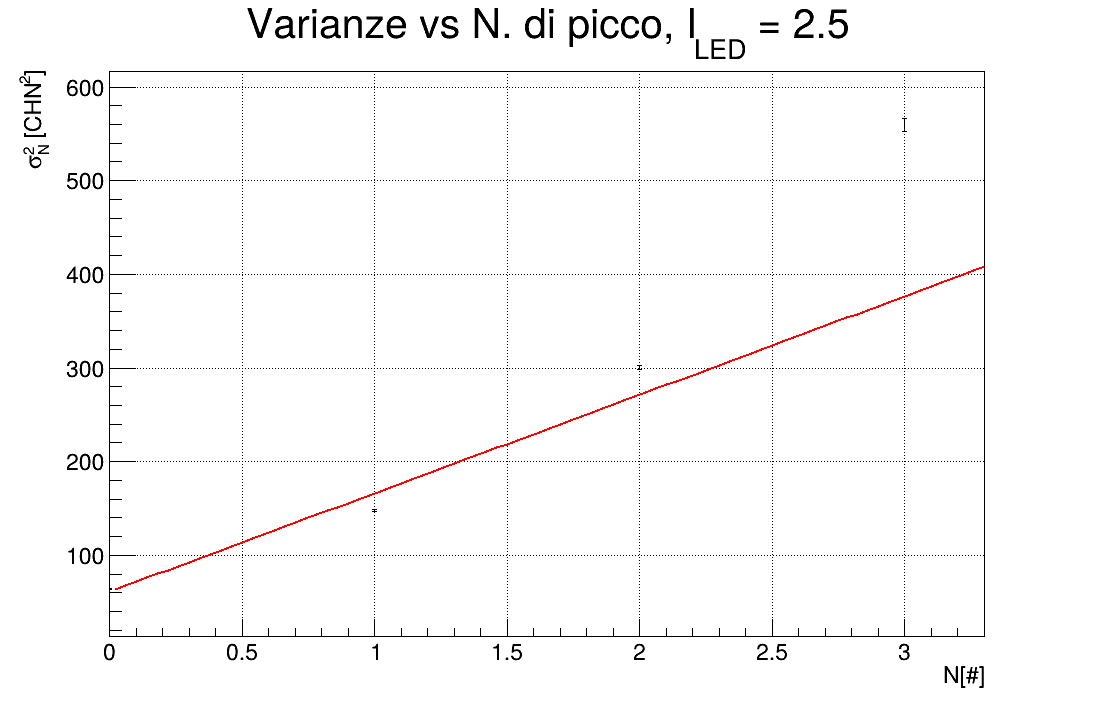
\includegraphics[width=1.\linewidth]{fig1/led_var_2_5.png}
    \caption{ \footnotesize Grafico delle varianze delle gaussiane per lo spettro a $I_{LED} = 2.5$ in funzione del numero di picco con fit lineare non convergente, $\chi^2 = 1453$ e d.o.f$=2$.}
    \label{fig:led_var_2_5}
\end{figure}
\end{multicols}
Il fit lineare non va a buon fine in nessuno dei tre casi, probabilmente per una sottostima delle incertezze sulle varianze, stimate dalle incertezze sui parametri $\sigma_N$ delle gaussiane.

I grafici dello spettro eneregetico, dell'istogramma delle aree e del grafico delle varianze per gli altri due valori di $I_{LED}$ si trovano in appendice 5.2.4.